\chapter{Signal flow}
From the previous chapter, we know that the cellular machinery of 
transcriptional and metabolic regulation is under-represented in the strongly 
regulated genes and thus hidden from the time-resolved transcriptome data. 
Consequently, the investigation of strong responders only gives insights into
the periphery of the gene regulatory network and functions directly related
to the cellular phenotype. What is largely missing is a holistic picture of
the signaling pathway activity, namely how the external stimulus is translated
to the protein signaling events that propagate through the protein interaction
network and ultimately lead to the measured gene regulation (\ref{fig:signal_flow}).

\begin{figure}[!ht]
\begin{center}
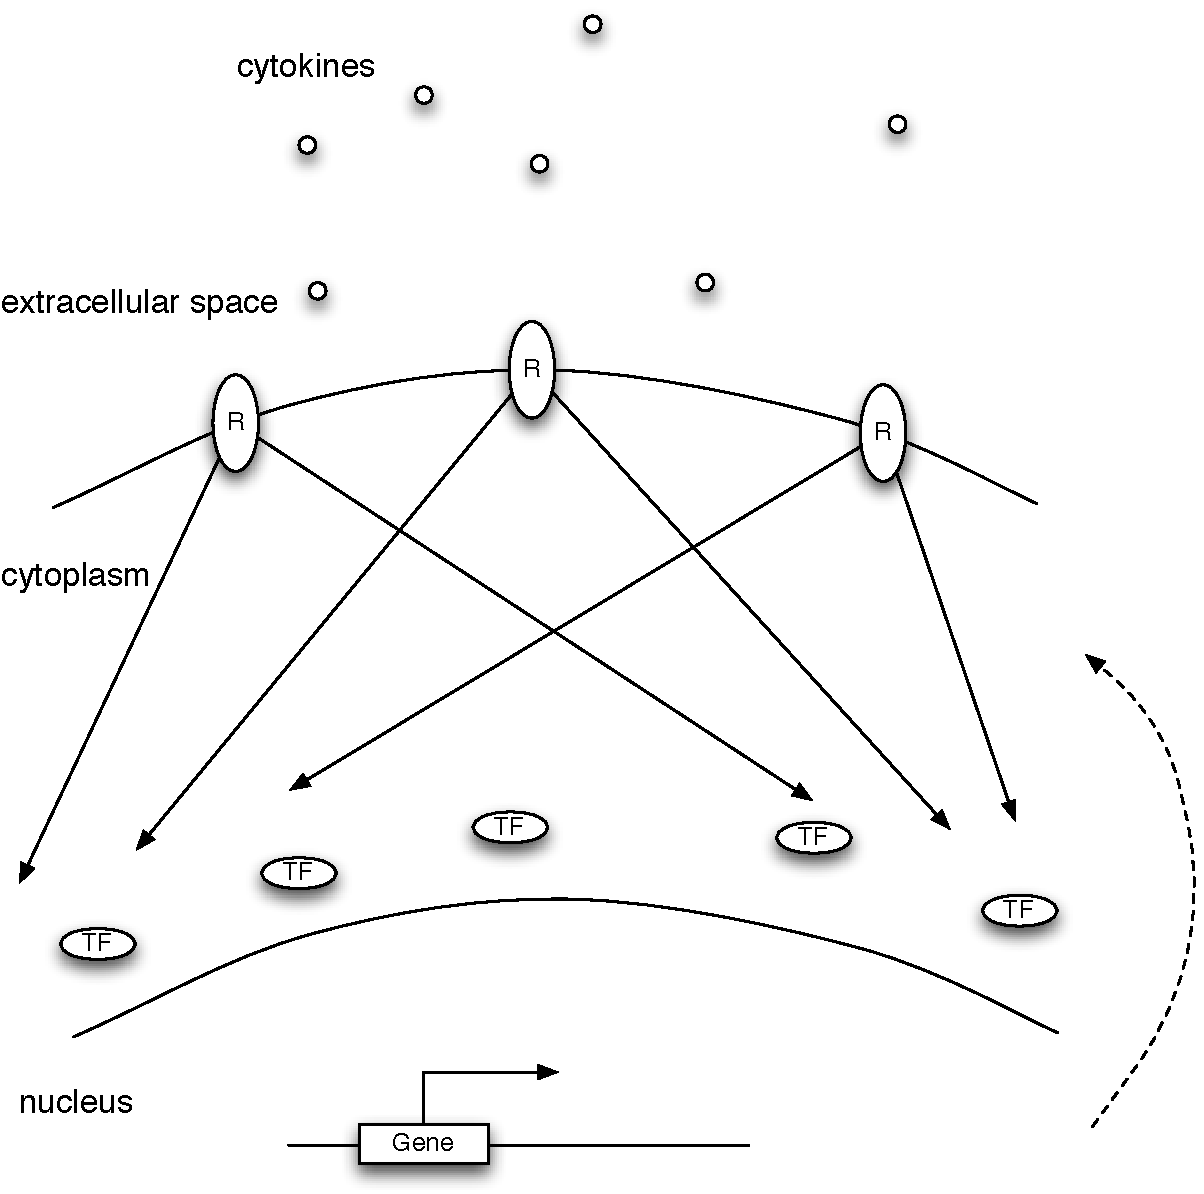
\includegraphics[width=\textwidth]{signal_flow.pdf}
\end{center}
\caption[Signal flow]{{\bf Schematic view of signal flow from membrane 
receptors to transcription factors in the cell.}
}
\label{fig:signal_flow}
\end{figure}

In the following, we first introduce several classical methods to infer the
enrichment of pathways from the transcriptome data. We point out the drawback
of their implicit assumptions and propose a two-step approach to identify the
causal signal\footnote{We use \emph{signal} and \emph{information} interchangably.} 
flow from membrane receptors to transcription factors. Finally,
we apply this approach in the study of cell-cell communication in the lung
cancer and skin.

\section{Pathway enrichment analyses}
Since the introduction of the microarray technology, pathway analysis has been 
a heavy focus and first choice for gaining insight into the underlying biology 
of differentially expressed genes. Over the past decade, we have seen at least 
three generations of pathway analyses~\citep{Khatri2012}, here we discuss 
their core features and limitations.

\subsection{Over-representation test}
Over-representation test is also called Fisher's exact test, it statistically 
evaluates the fraction of genes in a particular pathway found among the set 
of genes showing significant changes in expression. By constructing a
$2 \times 2$ contingency table, a researcher first chooses genes that are 
differentially over- or under-expressed in a given condition at a certain 
threshold. Then, for each pathway, the number of genes that are part of the 
pathway is counted. This process is repeated for an appropriate background 
list of genes (e.g., all genes measured on a microarray). Next, every pathway 
is tested for over- or under-representation based on this contingency table. 
The most commonly used test is based on the hypergeometric distribution or
the Fisher's exact test.

One of the critics on Fisher's exact test is that it only considers a ranked
list of differentially expressed genes and is thus independent of the 
measured fold changes. Second, the generation of the contingency table
requires setting a significance cutoff to count the number of differentially
regulated genes. This procedure introduces a subjective criterion and 
effectively treats the gene regulation as a black-white picture, namely only 
genes above this threshold are considered differentially expressed and those
below the threshold are then discarded.
    
\subsection{Gene set analysis}
To avoid the arbitrary significance cutoff and to realize the fact that weaker 
but coordinated changes in sets of functionally related genes (i.e., pathways) 
can also have significant effects, gene set enrichment analysis was suggested~%
\citep{Subramanian2005,Luo2009}. In general,
a pathway-level (gene group level) statistic is calculated from the gene-level 
statistic, and the statistical significance is assessed according to the 
pathway-level statistic.

By considering the coordinated changes in gene expression, gene set analyses 
account for dependence between genes in a certain pathway or group, however,
each pathway is still analyzed independently and thus crosstalks between
pathways are disregarded.

\subsection{Topology-based approach (SPIA)}
Over-representation and gene set analyses only consider the number of genes 
in a pathway to identify significant pathways, and ignore the additional 
information available from various prior knowledge bases. Recently a signaling
pathway impact analysis (SPIA) was proposed~%
\citep{Tarca2009}. SPIA considers the structure and dynamics of an entire 
pathway by incorporating changes in gene expression, types of interactions, 
and the positions of genes in a pathway. 
It calculates the pathway-level statistic from the combinatorial probability 
of perturbation in gene expression and over-representation. One obvious problem 
of the topology-based approach is that the true pathway topology is highly
context-dependent and remains poorly understood and annotated.

\subsection{NetSearch}
\cite{Steffen2002} further built upon the idea of incorporating 
prior knowledge about the pathway topology and suggested
the inference of signal transduction networks with protein-interaction maps
and expression profiles from DNA microarrays.
It works by first enumerating all possible linear paths
of a specified length through the interaction map starting
at any membrane protein and ending on any DNA-binding
transcription factors.
Microarray expression data are then used
to rank all paths according to the degree of similarity in
the expression profiles of pathway members.
Linear pathways
that have common starting points and endpoints
and of the highest ranks are then combined into the final
model of the branched networks.

Based on the gene expression data of pheromone response in the yeast, the 
NetSearch algorithm accurately reconstructs the MAPK cascade, it also identifies a 
network with other proteins necessary to execute the coordinated processes of 
growth polarization and cell cycle arrest, and reflects the complex topology of 
the interaction network in response to pheromone.

\subsection{Drawback}
All the above methods make the implicit assumption that the expression of genes
and their corresponding protein products are correlated, or the signaling 
pathway activity, which is largely determined by the member protein level, 
can be inferred from the transcriptome data. There has been ongoing debate 
about whether the transcriptome regulation correlates with the proteome
in bacterial and mammalian cells~\citep{Taniguchi2010,Ghazalpour2011}. More
often than not, the assumption of correlation either does not hold or is too 
strong. Therefore, questions arise about the validity of inferring signaling 
pathway activity based on the gene expression level.

\section{Two-step approach to causal signal flow}
We propose here a two-step approach to infer the activated protein signaling
pathways from time-resolved microarray data. As a first step, we apply a
gene set enrichemnt analysis to test the
enrichment of transcription factor target genes, which acts as a proxy of
the transcription factor activity \emph{per se}. Second, the upstream 
signal flow from membrane receptors to transcription factors is predicted 
based on the distance between both end nodes in the protein interaction
network.

\subsection{Identification of activated transcription factors}
We performed gene set enrichment tests, 
using a modified implementation~\citep{Luo2009}.
To this end, we retrieved sets of genes regulated by 
a common transcription factor from MSigDB v3.0 (The Molecular Signature Database). 
This database contains two major data sources. The first one is mammalian 
transcriptional regulatory motifs from the v7.4 public version of TRANSFAC 
database~\citep{Matys2003b}. We then generated the motif gene sets consisting 
of the inferred target genes for each motif. Every such set consists of human 
genes whose promoters (defined as regions -2kb to +2kb around transcription 
start site) contain at least one instance of the motif.
The second data source for transcription factor targets in MSigDB is derived 
from upstream motifs highly conserved among five mammalian species~%
\citep{Xie2005e}. Each motif gene set consists of all human genes whose 
promoters contained at least one conserved instance of the motif.

Individual genes were  ranked according to their response strengths as derived from the 
multidimensional scaling of the normalized time series 
(\ref{sec:response_strength}). 
The gene sets from MSigDB were  then tested for their enrichment 
 relative to the whole transcriptome by a Kolmogorov-Smirnov statistic. 

\subsection{Signal flow from membrane receptors}
In order to infer how extracellular signal flows from the membrane receptors to 
the transcription factors and subsequently induces gene regulation, it is 
crucial to be able to measure the proximity between a given pair of receptor and
transcription factor in the protein-protein interaction network. Here we 
compare two distance metrics, one is the shortest path length, and the other
being the mean first passage time based on the idea of random walk.

\subsubsection{Shortest path length}
If one assumes that information propagates in the network in a most parsimonious
or efficient way,
shortest path (SP) length between two nodes in the network is a classical way to
assess the distance between these two nodes and thus possible route of signal flow
(\ref{sec:shortest_path}).
We use a directed human protein-protein interaction network from a previous study%
~\citep{Vinayagam2011}, which contains edge directions
inferred by a naive Bayesian classifier.
For each cytokine receptor/transcription factor pair previously identified,
we calculated the length of the shortest path between the two
using the unweighted breadth-first search algorithm,
as implemented in the R package \texttt{igraph}~\citep{Csardi2006}.
We use these lengths as base metric for the probability 
of signal actually flowing through the pathway.

Intuitively, the shortest path is only the best scenario of all possible routes
of information flow in the network. Therefore, it simply ignores the 
neighborhood or global structure around the shortest path when calculating
distances. Another limitation of the shortest path distance metric has to do
with the small characteristic path lengths in a small-world networks~%
\citep{Watts1998}, such that any nodes can be reached from any other nodes
within only few hops when traveling on the shortest path and the shortest path
metric loses its discriminative power. Since most biological
and real-world networks demonstrate the small-world feature~%
\citep{Barabasi2004}, this limitation
has to be kept in mind when working with the shortest path.

\subsubsection{Mean first passage time}
The mean first passage time (MFPT) is defined as the average time/steps 
necessary for 
a random walker starting from a source node to reach a target node for the
first time. It has been shown that MFPT can be used to detect community
structures in the protein interaction network of yeast~\citep{Zhou2003}. 
Recently, a random walk with restart approach was applied to associate
target gene sets to reference datasets as an alternative to 
over-representation-based enrichement analyses~\citep{Glaab2012}. Furthermore,
the usefulness of MFPT became evident by the fact that the pairwise MFPT 
matrix is sufficient to reconstruct the full network topology~%
\citep{Wittmann2009}.

MFPT can be calculated analytically by solving a linear equation system~%
\citep{Kampen2007}. Consider the special case of a linear chain 
(\ref{fig:mfpt_calculation}) and suppose the random walker starts from node 
$x$ at a certain time $t$, with the probability of jumping to adjacent nodes
being equal, we have
\begin{equation}
\tau(x,y) - 1 = \frac{1}{2}\tau(x-1,y) + \frac{1}{2}\tau(x+1,y)
\label{eq:mfpt}
\end{equation}
where $\tau(x,y)$ denotes the mean first passage time of reaching $y$ and 
starting at $x$, which can be decomposed of 1 time unit needed to reach the
next time step $t+1$ and the travel time to the target node $y$ at $t+1$.
Since the random walker can be at either node $x-1$ or $x+1$ at $t+1$, each
with equal probability, we express the mean first passage time to $y$ at
time step $t+1$ as the right-hand-side of \ref{eq:mfpt}.

\begin{figure}[!ht]
\begin{center}
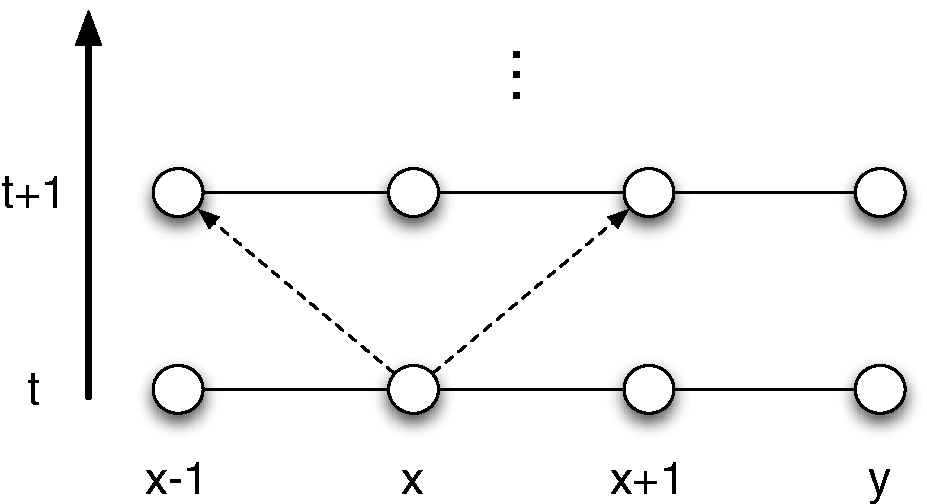
\includegraphics[width=\textwidth]{mfpt_calculation.pdf}
\end{center}
\caption[MFPT calculation]{
{\bf The calculation of MFPT on a linear chain.}
The same linear chain consisting of 4 nodes is depicted in different time 
slices ($t,t+1,\ldots$), 
a random walker starting from node $x$ at time $t$ can jump to either $x-1$ 
or $x+1$ at time $t+1$.
}
\label{fig:mfpt_calculation}
\end{figure}

\ref{eq:mfpt} can be rewritten and generalized to an arbitrary graph, i.e.
the mean first passage time from all possible nodes to a target node $y$
can be expressed as a linear equation system
\begin{equation}
(\tilde{\mathbf{L}}-\boldsymbol{\beta}^y) 
\begin{pmatrix}
\tau(1,y)\\
\tau(2,y)\\
\vdots\\
\tau(N,y)
\end{pmatrix}
= \boldsymbol{\delta}
\label{eq:mfpt_system}
\end{equation}
where 
\begin{equation}
\delta_i=
\begin{cases}
0 & i=y\\
1 & \textnormal{otherwise}
\end{cases}
\end{equation}
and $\tilde{\mathbf{L}}$ is the normalized graph Laplacian and
\begin{equation}
\tilde{L}_{ij}=
\begin{cases}
1 & i=j\\
-1/deg(i) & i \neq j \ \textnormal{and}\ i \ \textnormal{is adjacent to}\ j \\
0 & \textnormal{otherwise}
\end{cases}
\end{equation}
where $deg(i)$ is the degree of node $i$. $\boldsymbol{\beta^y}$ 
is the boundary condition
matrix that ensures $\tau(y,y)=0$, more specifically
\begin{equation}
\beta^y_{ij}=
\begin{cases}
\tilde{L}_{ij}-1 & i=j=y\\
\tilde{L}_{ij} & i=y\\
0 & \textnormal{otherwise}
\end{cases}
\end{equation}
It is easy to see that $\tilde{\mathbf{L}}$ can be pre-calculated and then be 
reused to estimate the
MFPT for each target node $y$. Moreover, the calculations
for different targets are independent and hence can be
determined in parallel. As networks in biology are often
sparse, the equation system in \ref{eq:mfpt_system}
is suitably represented by a sparse matrix. The matrix
is positive semi-definite and can be solved by the LGMRES algorithm~%
\citep{Baker2005}.

\ref{fig:mfpt_toy} compares the distance measure of shortest path (SP) length
and mean first passage time (MFPT) on different toy networks. Network A, B and
C are all composed of a linear chains as the backbone and different complex 
global structures, the SP metric measures the length of the backbond and is 
thus the same across all three topologies, whereas MFPT has a broader range
and changes between 9 and 17.5. This demonstrates that SP does not take into
account the global network topology. Furthermore, SP is also more susceptible
than MFPT to the pruning of a critical link, which is illustrated in the 
network C and D with only a single connection between $n1$ and $n2$ removed
in D. Since this edge is part of the shortest path between $n0$ and $n3$, the
SP distance changes dramatically by 33\%, while MFPT increase only moderately
by 3\%.

\begin{figure}[!ht]
\begin{center}
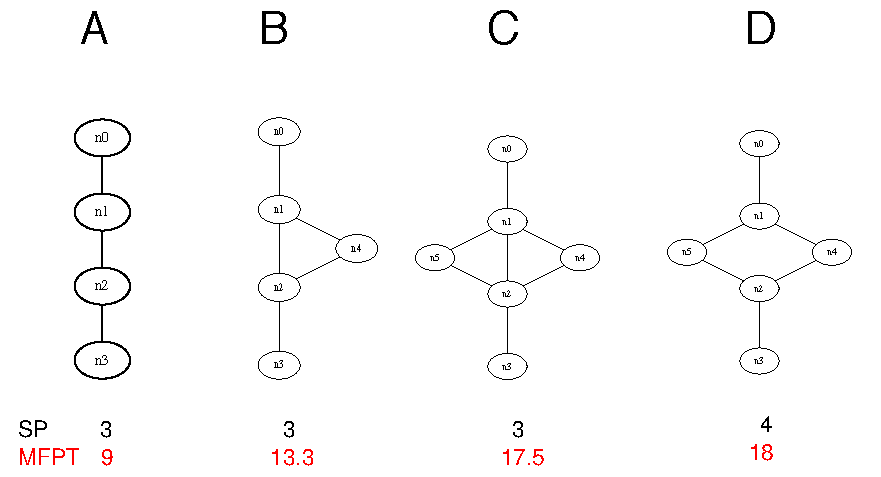
\includegraphics[width=\textwidth]{mfpt_toy.pdf}
\end{center}
\caption[Toy example of SP and MFPT on different topologies]{
{\bf Comparison of shortest path (SP) length and mean first passage time 
(MFPT) on different toy networks.}
Shown are the distances between node $n0$ and $n3$ measured in shortest path 
(SP) and mean first passage time (MFPT) respectively.
}
\label{fig:mfpt_toy}
\end{figure}

\section{Application in tumor-stroma interaction of lung cancer}

The hallmark of lung tumor development is its early spread, 
complicating the patient treatment and strongly impairing survival.
Recent studies have shown the tumor-stroma interaction to be relevant to 
tumor growth and spread, and therefore a possible target for
novel, effective treatment. 
However, 
the details by which tumor and stroma cells communicate remain poorly 
understood. In this section we present a study
of the migration mechanisms of a non-small-cell lung 
tumor cell line (H838) under the influence of endothelial (HPAEC) cells 
in a coculture system.

To obtain a holistic overview of the migratory processes, 
we recorded the time-resolved changes in the transcriptome of tumor cells
in scratch assays of aforementioned cocultures, and measured
cytokine concentrations in the medium.
H838 showed a significantly increased migration area after 24h in the 
H838/HPAEC coculture compared to the H838/H838 coculture.
Two cytokines, TNF-$\alpha$ and SDF-1$\alpha$, were shown to directly 
induce migration, 
and the transcripts of these two key factors were regulated only 
in HPAEC cells.
Gene set enrichment test identified coordinated regulation
of transcription factors targets
that cause the transcriptome response in H838. 
We compared distances from the cytokine receptors to the predicted
transcription factors using both shortest path and mean first passage time.
%suggests that TNF-$\alpha$ receptors activate multiple
%downstream targets in a homogeneous fashion,
%whereas the shortest paths \change[JB]{between}{descending from} 
%the SDF-1$\alpha$ receptor
%have multiple characteristic path lengths. 
%We conclude that TNF-$\alpha$ induces \change[JB]{the sustained}{an unspecific} 
%activation 
%of various downstream transcription factors, 
%which is the \change[JB]{primary}{initial} response \remove[JB]{mechanism} 
%involved in the 
%migration of H838 cells. 
%At the same time, the delayed activation of SDF-1$\alpha$ induce\change[JB]{d}{s 
%specific} pathways 
%\add[JB]{that} could provide a fail-safe mechanism.

\subsection{Background}
Lung cancer with its predominant type non small cell lung carcinoma 
(NSCLC) is the leading cause of cancer-related mortality worldwide.
The hallmark of lung cancer is its early spread, 
making it particularly dangerous, with associated high rate of death 
and short survival.
Whether this is an inherent feature of the non-small cell 
lung tumor cells or 
due to their microenvironment is still unknown. 

Ever since the formulation of \emph{seed and soil} theory by the English 
surgeon Stephen Paget in 1889~\citep{Paget1889}, there has been increasing 
interest in studying the tumor-stroma interactions. 
It is now largely acknowledged that sites of metastasis are determined 
not only by the characteristics of the tumor
cells but also by the microenvironment of
the host tissue~\citep{Fidler2003}. Tumor cells can generate a supportive
microenvironment by producing stroma-modulating
growth factors, which act in a
paracrine manner to induce stromal reactions such as
angiogenesis~\citep{Bergers2003}
and inflammatory response~\citep{Coussens2002}. Stroma cells in turn can
interact with primary tumor cells synergistically and facilitate their migration~%
\citep{Wyckoff2004}.
Stromal cells also make promising drug targets, since they are not as 
genetically
unstable as cancer cells, and are therefore less likely to
develop drug resistance~\citep{Kerbel1997}. To date, a number of drugs targeted
at tumor microenvironment, i.e. endothelial cells, immune cells and components
of the extracellular matrix, are at different stages of clinical 
trials~\citep{Mueller2004}. However, side effects of such stroma-targeting drugs
have also been observed, which raises the natural demand of a more detailed, 
systematic understanding of the tumor-stroma interaction.

While bearing in mind that tumor-stroma interactions can be mediated by direct cell-cell contact or modification of the extracellular matrix
components~\citep{Micke2004a}, most studies have focused on the tumor-stroma interaction through
single soluble factors~\citep{Kryczek2007,Saijo2002i,Nakamura1997}. 
\cite{Zhong2008} identified cytokines that are crucial for the 
tumor cell proliferation
and stromal cell migration by screening the whole secretome from
an adenocarcinoma/stromal murine lung cell coculture.
\cite{Sato2004} studied
the transcriptome homeostasis of pancreatic
cancer cells and stromal fibroblasts,
and singled out candidate genes that are
differentially expressed in coculture.
One of the most important types of stromal cells are endothelial cells (EC), 
the integral components of blood vessels. ECs not only promote the homeostasis of 
vascular system, but play an important role in tumor progression as well. 
It was shown that ECs influence different responses of cancer cells, such as 
proliferation and invasiveness \emph{in vitro}, as well as the metastatic potential 
of tumor cells \emph{in vivo}~\citep{Franses2011}.

Here, we combine the previous approaches and
study \emph{in vitro} the crosstalk between tumor and 
endothelial cells in  a non-small-cell lung cancer model: namely,
H838 lung cancer cells and HPAEC, i.e. human pulmonary artery endothelial cells.
We found that the  migration of  H838 cells in a trans-well H838/HPAEC coculture
was significantly enhanced when compared to monoculture.
Gene set enrichment analysis of the dynamic transcriptome
response of the H838 cells  revealed a coculture specific response 
that correlated with enhanced migration.
A cytokine array and subsequent single factor stimulation
identified the cytokines \tnfa and \sdfonea
to be the main factors enhancing H838 cell migration,
being \emph{de novo} expressed and originating in the endothelial cells alone. 

We further 
traced causes of the transcriptome response in the tumor cells back to the
\tnfa and \sdfonea receptors. % via the transcription factors and upstream protein signaling.
%We identified the dynamic regulation pattern of transcription factors. 
Assuming that cellular signal is most likely transmitted through the shortest 
path in a protein-protein interaction network, we 
mapped the putative pathways linking cytokine receptors with the 
transcription factors evoking the transcriptome response. 
%Based on \change[JB]{the above}{our results}, we hypothesize that \tnfa receptor family 
%members are likely associated with a wide spectrum of transcription factors, which
%renders the \tnfa-induced pathway an unspecific response in the first place.
%On the other hand, the \sdfonea receptor CXCR4 
%preferentially activates transcription factors such as 
%STAT3/6, LMO2, HSF1, IRF2, JUN/FOS, which are predominantly 
%enriched between 12 and 16 hours after coculture and represents a fine-tuned
%secondary activity leading to migration. \note[SD]{Should we mention the purpose of the paper in few sentences?}

% We need some concluding sentence here wraping up teh biology


% Results and Discussion can be combined.
\subsection{Results}

\subsubsection{H838 migration rate is enhanced in a transfilter co-culture with HPAEC cells}

To investigate the changes in migration behavior of lung tumor cells under the 
influence of stromal cells we cultivated  
H838 cells  together with either human pulmonary artery endothelial cells (HPAEC) or additional H838 cells in a trans-filter system (\ref{fig:migration} A).
The experimental setup of the homo- and heterogeneous cocultures ensured 
similar physical and environmental conditions, thereby minimizing 
experimental artifacts, e.g. due to different cell numbers per conditions. 

\begin{figure}[!ht]
\begin{center}
\includegraphics[width=\textwidth]{fig-migration.pdf}
\end{center}
\caption[H838 migration in homo- and heterogeneous coculture]{
{\bf Migration of H838 cells in the homo- and heterogeneous coculture.} 
(A) Trans-filter system. (B) Scratch assay of the homo- and heterogeneous coculture.
(C) Migration area of H838 cells at 24h after scratch from multiple independent 
experiments 
plotted as 
boxplots for the homogeneous (H838 + H838) and heterogeneous (H838 + HPAEC) 
coculture.
}
\label{fig:migration}
\end{figure}

Tumor cells on the bottom of the cell culture dish were scratched and the 
closing of the cell-free area was observed using time-lapse microscopy, in both
homo- and heterogenous cocultures (\ref{fig:migration} B).
In the heterogeneous cocultures, 
H838 cells close on average $963.5\pm156.8\ \mu m^2$ 
(mean $\pm$ standard deviation) within 24h, 
against $702.8\pm104.0\ \mu m^2$ in the homogeneous cocultures 
(\ref{fig:migration} C). 
% Note that we should put all these figures into one panel 
The migration area of the heterogeneous cocultures is significantly higher, and
a two-sided  $t$-test of the difference observed yields a $p$-value of 
$2.82 \times 10^{-5}$.

\subsubsection{Transcriptome response of H838 cells}
To explore the mechanisms leading to the enhanced cell migration, we recorded the time-resolved transcriptome response of the tumor cells during migration.
Illumina Human HT-12 Expression BeadChip was employed to compare the dynamic transcriptome response of scratched H838 cells in both homo- and heterogenous coculture conditions.
We collected mRNA at $t=(0,0.5,1,2,3,4,5,10,15,24)h$ after scratching for microarrays,
the data of which were quantile-normalized~\citep{Dunning2008a}.  
Discarding lowly expressed probesets and those with low interquartile 
variability between samples, we finally mapped the probes to 14922 EntrezID 
annotated genes. 
% Here we should show a time-resolved GO analysis or something similar (Fig. 2)
% Also add the analysis in the materials and methods
We analyzed the basal differential gene expression between homo- and
heterogeneous coculture by linear model fitting and Bayesian variance estimation~%
\citep{Smyth2004}, as well as the dynamic differential gene expression by fitting
the time series with a full/reduced polynomial model~\citep{Mar2009}. At 0h, only 2
genes are significantly down-regulated in the homogeneous coculture with respect
to the heterogeneous coculture (\ref{fig:transcriptome}A), 
and their absolute log fold changes are less than 1. Over time, there are more
genes classified as significantly up- and down-regulated by comparing the full and
reduced model fitting (Fig.~\ref{fig:transcriptome}B). Nevertheless, none of genes
has an absolute
average log fold change that exceeds 1. Taken together, the majority of genes
in H838 cells are not differentially expressed in the homo- and heterogeneous
coculture conditions. In order to take a glance at what is the function of those
differentially regulated genes, and to overcome the difficulty in detecting weak
but simultaneous regulation, we analyzed the transcriptome data with gene set
enrichment test~\citep{Luo2009}.
The enhancement of cell migration correlates with the differential upregulation 
of cancer and metastasis related gene sets at the basal level (Table 1). 
There are more number of, but less specific downregulated gene sets, which range
from metastasis, to aging and apoptosis (Table 2). 

\subsubsection{Supernatant  from different co-cultures show distinct cytokine composition}

To identify the cytokines that mediate the communication between
HPAEC and H838 cells and enhance the tumor cell migration,
we quantified the cytokine composition
of the  homo- and heterogeneous cocultures
both before and 24h after onset of migration.
We used a  fluorescent bead array based cytokine assay which detects fifty cytokines
(see Materials and Methods and Table S3).
A total of twenty-four different cytokines were present in detectable amounts,
fifteen of which showed significant differential upregulation
(\ref{fig:cytokine} A).
% Should add here an additional table with the quantification of all cytokines
Gro-$\alpha$, MCP-3, IL-6, IL-8, IL-13, FGF basic, G-CSF, IP-10 and RANTES were
upregulated in the heterogeneous coculture prior to cell migration \remove[JB]{and
remained unchanged with respect to the unscratched control}.
MIF, IL-12, IL-15, MCP-1 and TNF-$\alpha$ were also upregulated
in the heterogeneous cocultures, \change[JB]{but}{and} this upregulation \change[SD]{increased}{was increasing}
during tumor cell migration.
Finally, SDF-1$\alpha$ was only found in the heterogeneous coculture,
and was also upregulated after scratching. 

% Need a better headline for the subsection here 
\subsection*{Isolation of cytokines relevant to migration}

Based on the previous analysis, 
we selected seven cytokines that were differentially regulated  
during tumor cell migration 
% need some idea why we did not add MIF to the candidate list
(TNF-$\alpha$, IL-6, RANTES, SDF-1$\alpha$, MCP-1, IL-8, Gro-$\alpha$).
Furthermore, we added VEGF as cytokine candidate for its known involvement in
angiogenesis and metastasis of tumor cells~\cite{Ferrara2003,Hiratsuka2002} 
\remove[JB]{and 
because the GSEA analysis revealed angiogenesis to be a
differentially regulated gene function of migrating H838 cells in 
coculture conditions}.

To test the influence of the above factors on tumor cell migration,
we analysed scratch assays of H838 monocultures under the influence of 
individual or multiple of these cytokines. 
Comparing migration areas after 24h, 
we found that only IL-6, TNF-$\alpha$ and SDF-1$\alpha$ significantly 
increase the migration of H838 cells (Fig.~\ref{fig:cytokine}B, two-sided $t$-test,
$p < 0.05$). 
To further corroborate this result, we neutralized 
TNF-$\alpha$ and SDF-1$\alpha$ in heterogeneous cocultures  by adding neutralizing antibodys (cf. Material and Methodes)
Inhibition of  either TNF-$\alpha$ or SDF-1$\alpha$ significantly reduced tumor cell migration (Fig.~\ref{fig:cytokine}C). 
Simultaneous inhibition of TNF-$\alpha$ and SDF-1$\alpha$ did not result in an additive effect, yet increased the statistical significance of the migration 
\add[JB]{inhibition} 
(two-sided $t$-test, $p=1.6\times10^{-4}$).

\subsection*{Cytokine genes are expressed differently in H838 and HPAEC}

To elucidate the origin of the differential cytokine concentrations,
we assumed an implicit correlation between gene expression and protein abundance.%
\note[JB]{ref?}
Under this hypothesis, it is to be expected that gene expression profiles of
H838 cells will be such that 
our previously identified cytokines of interest should be differentially 
expressed between homo- and heterogenous coculture conditions.
We compared the basal 
expression levels of all genes with protein products
annotated as cytokines in the KEGG cytokine-cytokine receptor interaction pathway. 
However, none of the cytokine encoding genes 
showed a differential basal regulation between the two coculture conditions 
(Fig.~\ref{fig:transcriptome}A). Over time, IL6 and CXCL14 are significantly
down-regulated, and CSF1 is significantly up-regulated. 
(Fig.~\ref{fig:transcriptome}B).
Both \tnfa and \sdfonea do
not respond differentially during H838 migration (Fig.~\ref{fig:cytokine_dynamic}A)
% maybe put this figure into the supplement
\change[JB]{O}{Looking at the basal expression levels within each culture condition, o}nly five out of 162 cytokines (IL18, IL10, PDGFC, BMP7 and TNFSF12) 
\remove[JB]{even} had a significantly high expression level in both conditions
(Fig.~\ref{fig:cytokine_basal}), 
and none of these could be directly related to the migration-enhancing 
cell-cell communication.\note[JB]{too strong}

We conclude that differential cytokine regulation in the supernatant 
must originate primarily from the HPAEC cells.  
A\add[JB]{n} RT\add[JB]{-}qPCR experiment confirmed an early and transient response of  
TNF-$\alpha$ as well as a later and prolonged upregulation of 
SDF-1$\alpha$ (Fig.~\ref{fig:cytokine_dynamic}B). 
Fitting the time course with an impulse model, which measures \add[JB]{the peak 
duration as} the 
temporal difference between \change[JB]{two}{the} inflection points \add[JB]{of two
sigmoidal curves} (cf. Materials and Methods), 
% add this in materials and methods
we obtain an activation duration of  8.3 hours and 1.6 hours for SDF-1$\alpha$
and TNF-$\alpha$, respectively.

\subsection*{Identification of putative transcription factors in the H838 gene expression}

Admitting the cell-cell communication from HPAEC to H838 cells 
via the  mobility factors TNF-$\alpha$ and SDF-1$\alpha$,
we sought to explain how is the
information transferred from the cytokine receptors to the gene expression. 
THIS NEEDS REWRITING. THE CLAIM TO NONTRIVIALITY AND TIMESCALES SEEMS TO BE
UNNECESSARY
The answer, in the form of pathways downstream from these key  cytokines, is made non-trivial by the fact that
transcriptome and secretome regulation changes have different time scales~\cite{Busch2008}. 
For this we trace the cause of the transcriptome dynamics back to the above identified cytokines via putative transcription factors, protein-protein interaction
and receptor activation. 

We applied a gene set enrichment test for the gene expression at 
the different time points using the transcription factor target gene sets~%
\cite{msigdb}.
The differential regulation of the gene sets was measured through
a PCA-like projection. We divided the 24h measurement time window 
into six intervals of four hours each,
wherein  we tested the enrichment of different 
transcription factor target genes. Within each time window, 
genes were ranked according to their differential response
kinetic between the homo- and heterogenous coculture responses. 
THE FOLLOWING NEEDS REWRITING. I HAVE STRUCK THIS MULTIDIMENSIONAL SCALING
BEFORE, AND IN ANY EVENT THIS LEVEL OF DETAIL SHOULD GO INTO THE METHODS
As a rank measure, we fitted the 2D projection from the multidimensional 
scaling~\cite{Strickert2009} and fit the resulting distribution with multivariate 
skew 
normal distribution to assign a p-value to each gene. % is this correct?
A non-parametric Kolmogorov-Smirnov test is subsequently performed for each
transcription factor target gene set within a certain time window compared to the 
background set.

Hierarchical clustering \add[JB]{of the enrichment score for different transcription 
factor targets
over time} identifies four  major clusters \remove[JB]{according to temporal 
enrichment of transcription factor target genes}: cluster A contains aryl 
hydrocarbon receptor (AHR) targets, which  are \add[JB]{significantly}
overrepresented after 16h and remain outliers due to this distinct 
enrichment pattern; 
\change[JB]{genes}{targets} of the AP1 complex (JUN, FOS) are induced between 
four and eight hours and
are part of the cluster B; cluster C includes transcription factors 
\change[JB]{that}{whose target genes} are mainly 
active between 12 and 24h, such as the viral oncogene homolog MYC;
\change[JB]{F}{f}urther transcription factors like  NFKB, STAT3/6, IRF2, 
that are known to play a role in
immune or cytokine response ~\cite{Hayden2008,Shuai2003,Wang2002} ,
\change[JB]{are induced}{induce the expression of their target genes}  
between twelve and sixteen hours. \add[JB]{Therefore, applying the gene set
enrichment method on the time-resolved microarray data, we identified here the
sequence of enriched transcription factor targets, which could also serve as
a proxy for the temporal activity of transcription factors \emph{per se}.}

% we need a concluding sentence here

\subsection*{Data-mining the pathways from cytokine receptors to transcription factors and gene response}

%\NOTE{THIS IS VERY QUESTIONABLE: After identifying the key cytokines as well as the transcriptional regulators  involved in the migration of H838 cells, it still remains largely unknown how the signal 
% flows between the corresponding cytokine receptors and the transcription factors  inferred from the transcriptome data.  DID WE? HOW? HOW DO THESE ABOVE CORRELATE IN TIME TO THE QPCR PROFILES? ARE THEY BIOLOGICALLY RELEVANT? WHERE IS THIS INFORMATION? HOW DOES ONE INFER THAT THE RESULTS FROM THE MICROARRAY CORRELATE TO  MIGRATION? IF THEY DO, IS IT CAUSAL? IF SO, IN WHICH DIRECTION?} 

To further bridge the gap between the transcription factors identified above and TNF-$\alpha$, SDF-1$\alpha$, or even other cytokines not investigated in this
study, we mapped shortest paths from each cytokine receptor to all putative transcription factors, using a directed protein-protein
interaction network~\cite{Vinayagam2011}.  Results are summarily  illustrated in Fig.~\ref{fig:shortest_path}.

% How is the length measured? How do we quantify?
% BY WHAT CRITERIA? HOW IS LENGTH MEASURED? HOW CAN LENGTH BE MEASURED, I.E. WHAT INFORMATION IS THERE ON THE NODES AND EDGES  DATABASE THAT CAN BE USED AS METRIC?

\remove[JB]{For TNF-$\alpha$ receptors % Agree with Gustavo, which ones exactly ?, 
we found several  pathways, of having similar shortest paths between the receptor and the putative TFs. 
Some prominent  shortest paths include those to FOS, NFKB and STAT3.
In contrast, the receptor for SDF-1$\alpha$, CXCR4 has a dominating  shortest path to only STAT3, 
implying the SDF-1$\alpha$ signal can only be transduced downstream when STAT3 regulated targets are active, 
which is between twelve and sixteen hours. 
In addition, we observed similar shortest path length patterns for IL8 and IL6 receptors, where the former has a more
uniform distribution of shortest path length and the latter is
highly biased towards only one transcription factor.}
% WHAT SIMILARITIES ARE TO BE OBSERVED, BETWEEN WHICH PLOTS IN THE FIGURE?}
%\mbox{} \leaders\vrule height 2.5pt depth -1.5pt \hfill \null

As depicted in Fig.~\ref{fig:shortest_path}A, 
the average shortest path distances from the TNF receptor super family 
members to the identified transcription factors have a dominant 
unimodal distribution 
(Hartigans' dip test~\cite{Hartigan1985}, $p=0.06073$) with a peak at 3.7, 
implying that the signal from the TNF receptors traverses 
the network in a homogeneous manner, through many equally likely paths
with a length of 3.7 on average. On the other hand, the shortest path lengths 
starting from the \sdfonea receptor,  CXCR4, have a significantly 
multimodal distribution (Hartigans' dip test,  $p=0.0007187$), 
or put differently, the signal downstream of CXCR4 prefers to travel 
through heterogeneous routes with different characteristic path lengths.

\change[JB]{Hierarchical clustering}{Principal component analysis and $k$-means 
clustering} of all the shortest path lengths between receptors
and transcription factors gives a systematic overview of the signal flow
pattern (Fig.~\ref{fig:shortest_path}B).
\change[JB]{A total of 3 clusters of receptors can be identified. 
THIS IS INFORMATION THAT SHOULD BE AT THE FIGURE'S CAPTION, AT LEAST SOME OF IT,
OR IN THE FIGURE ITSELF.
Five cytokine receptors,
CCR9, XCR1, IL22RA1/2 and IL11RA, have in general a large distance to all
putative transcription factors, and are thus less likely to transmit the cytokine
signal and determine the migration decision of H838 in our set-up.
CXCR4 belongs to the cluster with 3 separable vertical gray-scale  strips,
which is in line with the multimodality of CXCR4-originated path lengths.
Lastly,  TNFR is classified into the third cluster with more homogeneous
distance (color) pattern, which corresponds to the unimodality of TNFR-originated
path lengths.}{Different receptors are clustered in the space spanned by the first
and second principal components, which explain 76.7\% and 6.1\% of the total 
variance respectively. At a given resolution, TNFR and CXCR4 can be grouped into
different clusters, which corresponds to the uni- and multimodality of their shortest
path length distributions. In summary, the TNF-$\alpha$ and SDF-1$\alpha$ 
receptors transmit
information in a homo- and heterogeneous manner respectively, which could
possibly be generalized to other cytokine receptors.}

\section*{Discussion}

% THis needs to be filled with the ideas.

\remove[JB]{Taken together, we
hypothesize that there are at least two kinds of signal flows from the receptors
within the H838 cells in response to migration signals, a focalized and a fan-out 
activation of downstream transcription factors.}

\add[SD]{The key medical problem in lung cancer and its predominant type non-small 
cell lung carcinoma (NSCLC) is an early systemic metastatic spread of tumor cells 
independent of tumor size, which leads to high mortality rate. Tumor progression 
and metastasis is regulated by many different processes, inter alia by interactions 
via soluble factors between tumor cells and cells of tumor microenvironment, such as 
endothelial cells. In this study, we analyzed the interactions between NSCLC cells 
and endothelial cells and their influence on NSCLC cell migration. We identified 
two key cytokines, TNF-$\alpha$ and SDF-1$\alpha$, that are expressed by the 
endothelial cells and promote the migration of NSCLC cells.}

\add[JB]{In this study, we verified that TNF-$\alpha$ and SDF-1$\alpha$ are two
key cytokines that are expressed by the endothelial cells and promote the migration
of tumor cells. We proposed a two-step approach to link the transcriptome response
with the causal signal flow in the protein interaction network. First, gene set
enrichment analysis was applied to infer the sequence of transcription factor
activation that results in the gene expression. Second, we concluded from the 
shortest path in the interactome that 
TNF-$\alpha$ and SDF-1$\alpha$ receptors have different downstream signal flow 
pattern. We hypothesize that transient expression by endothelial cells initiates
an unspecific tumor cell response that transduces the signal along multiple
similar paths, whereas the delayed and prolonged expression of SDF-1$\alpha$ drives
the tumor cells to a more specific response that eventually determines the 
migration phenotype.}

Some ideas:\note[SD]{As next I would tell a few words about endothelial cell-tumor cell communication, what is known and what we found at transcription and protein level.
Then about the role of TNFa and SDF1a in tumors and lung tumors.
And finaly system biology}

\begin{itemize}
\item Discuss the contribution of proliferation/migration in scratch assay?\note[SD]{I would let it out. Normally mitomycin is given to migration assays to prevent proliferation. Dennis tested this, but found no difference in migration rate with or without mitomycin. Thats why he made his experiments without any proliferation inhibitors. If you think its important, we can include it in material and methods.}
The \emph{in vitro} scratch assay is a well established method
to study cell migration~\cite{Busch2008,Liang2007}, especially
in our experimental setting, the coculture of tumor and 
endothelial cells has no influence on the cell proliferation~%
\cite{Dauscher2012} and thus our results can be interpreted
as the net effect of tumor cell migration.

\item Discuss the non-autonomous regulation of H838 migration. It is very strange that only the endothelial cells do respond 
and secrete cytokines.

Nur die EC sezernieren ja nicht die Cytokine, sie werden ja auch von H838 sezerniert nur eben in geringeren Ma�en. 
\note[JB]{ref?}\note[SD]{Of course the tumor cells are secreting different cytokines to attract different stromal cells. But in this case not so much of SDF1 and TNFa}	

\item IS this related to early spread and metastasis in lung cancer? 

\item What do we know about Tnfa and SDFa with respect to cell migration?\\
\tnfa was first identified as an anti-tumor cytokine that is involved in the killing
of certain kinds of tumors, however, it is appreciated recently that \tnfa can also 
act as a tumor-promoting factor and enhance tumor growth and metastasis%
~\cite{Wu2010}. It has also been shown in the ovarian cancer cells cocultured with
macrophages that \tnfa can induce the up-regulation of 
CXCR4 mRNA, which is the receptor of \sdfonea. This response to \tnfa involves both
AP-1 and NF-$\kappa$B related pathways~\cite{Kulbe2005}. Blocking the \tnfa receptor
in mouse Lewis lung carcinoma cell cultures decreases the gene expression of CXCR4~%
\cite{Sasi2011}.

It has been shown that the \sdfonea/CXCR4 pathway has pleiotropic activities and it 
promotes tumor growth and malignancy, enhances tumor angiogenesis, participates in tumor metastasis, and contributes to immunosuppressive networks within the tumor microenvironment~\cite{Kryczek2007}. Both stroma and cancer cells can produce \sdfonea, 
although in our system it is mainly expressed by the endothelial cells. In the presence of neutralizing \sdfonea antibodies, NSCLC tumor metastases were also significantly reduced~\cite{Phillips2003}.

The identification of \tnfa as a key stroma-originating factor that promotes 
tumor cell migration is of great interest, since its release is a general response to chemotherapy in different stromal cell types~\cite{Acharyya2012}. Together with
other cytokines, such as HGF, that contribute to the drug resistance of cancer
treatment~\cite{Straussman2012}, these soluble factors in the tumor microenvironment
might be the key to the cancer therapy and the potential target of intervention.


\item What is new and what is known in the literature

\item What is new in our methods?\\
The advantage of our two-step approach to identifying signal flow in the protein 
interaction
network and relevant transcription factors that lead to the transcriptome response
is at least two-fold: first, we apply gene set enrichment test to avoid the hard 
significance cutoff in the conventional hypergeometric test and at the same time
to detect weak but coordinated regulation of transcription factor targets. This is 
necessary since the tumor cell transcriptome does not show significantly
differential regulation between the homo- and heterogeneous coculture 
(Fig.~\ref{fig:transcriptome}), which 
hints at a lack of correlation between the mRNA expression level and the protein 
activity. This in turn underlines the rationale behind the time-scale separation
in our approach. Second, due to the decoupling between the mRNA and protein
activities, it is vital to consider signaling pathways not directly represented
in the transcriptome data, but rather embedded in the protein interaction network
instead. In order to infer the signal flow from the membrane receptors to 
transcription factors, we simply assume that the signal traverses the shortest
path connecting a certain pair of receptor and transcription factor.

\item What new  biology do we find?\\
Based on our time-resolved qPCR results, we conclude that \tnfa in the endothelial 
cells is 
transiently expressed and peaks earlier than \sdfonea, whereas the latter has
a longer activation time window. These results are in line with the hypothesis 
that \tnfa induces the CXCR4 expression in tumor cells, which can then respond
to \sdfonea. Nevertheless, CXCR4 in the lung cancer cell line H838 is neither
basal highly expressed (Benjamini-Hochberg corrected $p$-value = 0.7977245), nor differentially regulated over time (Benjamini-Hochberg
corrected $p$-value = 0.893767) in the 
heterogeneous coculture of tumor and endothelial cells, which indicates that
cytokine receptors important for the communication with endothelial cells might
only be regulated at the protein level.

According to the transcription factor target enrichment analysis, target genes
of AP-1 are more significantly upregulated between 4 and 8 hours, whereas those
of NF-$\kappa$B are only activated between 12 and 16 hours, although both AP-1 and
NF-$\kappa$B are known to be involved in the \tnfa induced response~%
\cite{Kulbe2005}. Based on 
the early expression peak of \tnfa in the endothelial cells, it seems
in our particular coculture system of H838 and HPAEC cells, the initial 
transcriptome response in the tumor cells might be mediated through the AP-1
rather than the NF-$\kappa$B related pathway. It has also been
shown that the CXCL12/CXCR4 activation of NSCLC cell lines 
increased intracellular calcium mobilization and MAP kinase 
activation with enhanced ERK1/2 phosphorylation~%
\cite{Belperio2004}, which is 
known to be upstream of the AP-1 transcription complex.
Therefore, all evidence points to the important role of the
AP-1 complex in the tumor cells to convey the information of  
the \sdfonea/CXCR4 activation from the microenvironment.

By analyzing the shortest paths between receptors and transcription factors, 
we classified \tnfa and \sdfonea related 
pathways into the homogeneous and
heterogeneous response pattern respectively. Taking into account the different
expression dynamics of both cytokines in the endothelial cells, this implies a
complementary role \tnfa and \sdfonea play in the enhancement of lung cancer
cell migration. It could be that the transient expression of \tnfa by the 
endothelial cells initiates a first but unspecific response in the tumor cells,
while the secondary prolonged stimulation from \sdfonea leads to a signal that 
propagates preferentially 
on a more specific set of paths to the downstream transcription factors, which
ultimately determines \emph{point of no return} of the enhanced migration phenotype 
in the tumor cells.

\end{itemize}



\subsection*{Impulse model}
The qPCR time courses of \tnfa and \sdfonea measured in HPAEC cells are fitted with an impulse model~\cite{Chechik2009}, which is \remove[JB]{basically} composed of one rising and one falling sigmoidal curve, as defined by
\[
f(x) = \frac{1}{h_1} \cdot \left(h_0+\frac{h_1-h_0}{1+e^{-\beta_1(x-t_1)}}\right) \cdot
\left(h_2+\frac{h_1-h_2}{1+e^{\beta_2(x-t_2)}}\right), 
\]
where the three amplitude (height) parameters determine the initial amplitude 
($h_0$), the peak amplitude
($h_1$), and the steady state amplitude ($h_2$). The onset time $t_1$ is the time of  first transition (inflection point) and the offset $t_2$ is the time of second  transition. Finally, the slope parameters $\beta_1$ and $\beta_2$ determine the slope of the first and second transition. Parameters are estimated using a  Levenberg-Marquardt non-linear least squares  algorithm as implemented in the R package \texttt{minpack.lm}.

\subsection*{Calculating the significantly basal expressed genes}
In order to robustly estimate differentially regulated genes at the basal level and to avoid the commonly encountered 
presence of outliers and skewness~\cite{Marko2011}, we fitted 
a skew-$t$  distribution~\cite{Azzalini2003} to the $\log_2$ raw intensities at 0h. 
In addition to the regular $t$ distribution $f(x)$ with $v_{df}$ degrees of freedom, a skew-$t$ distribution,  $f_{skew}(x)$ has an additional 
skewing parameter $\gamma$ such that  
\[
f_{skew}\left(\frac{x-\xi}{\omega}\right) = 
\begin{cases}
\frac{2\gamma}{\gamma^2+1} \cdot f\left(\gamma\frac{x-\xi}{\omega}\right) & x<0\\
\frac{2\gamma}{\gamma^2+1} \cdot f\left(\frac{1}{\gamma}\frac{x-\xi}{\omega}\right) & x \geqslant 0\\
\end{cases}
\]
where $\xi$  and  $\omega$ denote the location and scale of the distribution.  
The basal level gene expression distribution was fitted using maximum likelihood 
estimation for the 
univariate skew-$t$ distribution, implemented in the R package \texttt{sn}.

\begin{figure}[!ht]
%\begin{center}
%\includegraphics[width=4in]{fig/h838-cytokine.pdf}
%\end{center}
\caption{
{\bf Differential basal and dynamic gene expression in homo- and heterogeneous 
cocultures.} 
(A) Volcano plot of the differential gene expression at 0h as determined by limma~%
\cite{Smyth2004}, the red dashed line
indicates the significance cutoff of $p = 0.05$.
(B) Volcano plot of the differential gene expression over time as determined by the
full/reduced model fitting~\cite{Mar2009}, the red dashed line
indicates the significance cutoff of $p = 0.05$.
}
\label{fig:transcriptome}
\end{figure}

\begin{figure}[!ht]
%\begin{center}
%\includegraphics[width=4in]{fig/h838-cytokine.pdf}
%\end{center}
\caption{
{\bf Identification of cytokines involved in the tumor cell migration.} 
(A) $\log_2$ transformed ratios of cytokine expression in heterogeneous respective
homogeneous coculture are shown. The black dashed line with a slope of 1 denotes 
the identity and the blue dashed lines denote the zero $\log_2$ fold change
or equal amount of cytokines between the scratched and unscratched conditioned 
media.
(B) Migration area of H838 cells at 24h after scratch in the H838 mono-culture 
treated with the 8
factors, the 2 factor groups and as in the control experiment.
(C) Migration area of H838 cells at 24h after scratch in the heterogeneous 
H838/HPAEC coculture 
treated with the neutralizing antibodies against TNF-$\alpha$, SDF-1$\alpha$
and both together. Asterisks in all plots denote that data are significantly 
different from the control according to a two-sided $t$-test ($p < 0.05$).
}
\label{fig:cytokine}
\end{figure}

\begin{figure}[!ht]
%\begin{center}
%\includegraphics[width=4in]{fig/cytokine-ex.pdf}
%\end{center}
\caption{
{\bf mRNA of TNF-$\alpha$ and SDF-1$\alpha$ is regulated in HPAEC instead of H838 
cells.}
(A) $\log_2$ fold expression of TNF-$\alpha$ and SDF-1$\alpha$ (CXCL12) in H838 
cells plotted
over time for the hetero- and homogeneous coculture respectively.
(B) $\log_2$ fold expression of TNF-$\alpha$ and SDF-1$\alpha$ in HPAEC cells 
from the qPCR
experiment in the heterogeneous coculture plotted
over time. Blue dashed lines denote the impulse model fit~\cite{Chechik2009}.
}
\label{fig:cytokine_dynamic}
\end{figure}

\begin{figure}[!ht]
%\begin{center}
%\includegraphics[width=4in]{fig/fig-plot_tfbs_modified.pdf}
%\end{center}
\caption{
{\bf Enrichment of transcription factor binding motifs over time as inferred
from the differential expression time course between hetero- and homogeneous
coculture.}
$-\log_{10}$ transformed $p-$values of the gene set enrichment test for 
different transcription factor binding motifs at each time window. Binding
motif names are the corresponding TRANSFAC matrix identifiers.
In addition, motifs highly conserved among 
five mammalian species~\cite{Xie2005e} are also included.  If the motif sequence 
matched no transcription factor binding site from TRANSFAC v7.4, then the gene set
is named as MOTIFSEQ\_UNKNOWN where MOTIFSEQ is the sequence of motif $m$.
}
\label{fig:gage}
\end{figure}

\begin{figure}[!ht]
%\begin{center}
%\includegraphics[width=4in]{fig/fig-sp_modified.pdf}
%\end{center}
\caption{{\bf Shortest paths between membrane receptors and transcription factors.}
(A) Distribution of shortest path lengths from TNFR and CXCR4 (\sdfonea receptor) to 
all predicted transcription factors. Ticks at the bottom indicate the actual data 
points, with a jitter of $[-0.2,0.2]$ added to increase visibility.
(B) PCA and $k$-means clustering of all cytokine 
receptors in the KEGG 
\emph{cytokine-cytokine receptor interaction pathway} based on their shortest paths
to all identified 
transcription factors in Fig.~\ref{fig:gage}.
}
\label{fig:shortest_path}
\end{figure}

\section*{Supporting Figure Legends}

\setcounter{figure}{0}
\makeatletter
\renewcommand{\thefigure}{S\@arabic\c@figure}
\begin{figure}[!ht]
%\begin{center}
%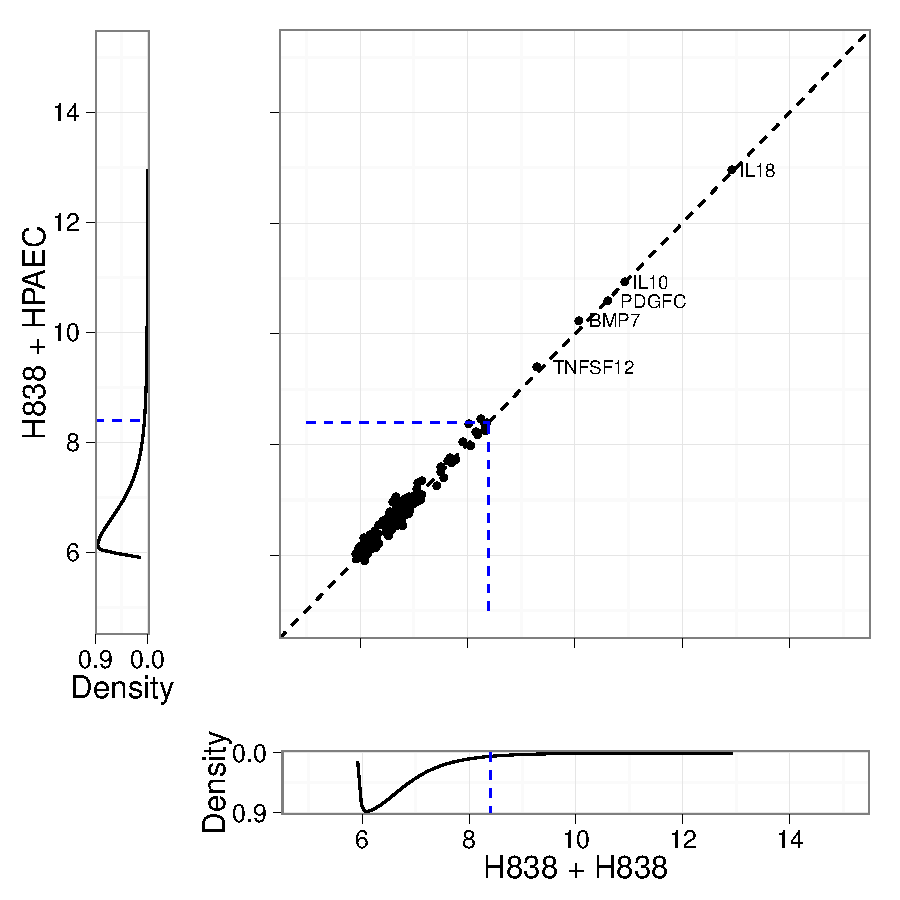
\includegraphics[width=4in]{fig/fig-basal_cytokine.pdf}
%\end{center}
\caption{
{\bf Few cytokines highly expressed in H838 at 0h.}
Comparison of $\log_2$ transformed basal mRNA intensities at 0h of all 
cytokines annotated 
in the KEGG \emph{cytokine-cytokine receptor interaction pathway} between
the hetero- and homogeneous coculture. Blue dashed lines denote the significance
level ($p=0.05$) after fitting the basal expression distribution with a skew-$t$ 
distribution~\cite{Azzalini2003}. Only IL18, IL10, PDGFC,
BMP7 and TNFSF12 are above this threshold in both conditions, 
i.e. significantly up-regulated
at 0h.
}
\label{fig:cytokine_basal}
\end{figure}

\makeatletter
\renewcommand{\thetable}{S\@arabic\c@table}
\section*{Tables}
%\begin{table}[!ht]
%\caption{
%\bf{Enriched GO terms among genes with top VIP scores}}
%\input{table_gage_up.tex}
%\begin{flushleft}Genes with a VIP score $>$ 1 within each time window are
%selected for the hypergeometric GO term enrichment test, and the top ranked
%GO categories with the least $p$-values are listed.
%\end{flushleft}
%\label{tab:go}
%\end{table}

%\begin{table}[!ht]
%\caption{
%\bf{Enriched GO terms among genes with top VIP scores}}
%\input{table_gage_down.tex}
%\begin{flushleft}Genes with a VIP score $>$ 1 within each time window are
%selected for the hypergeometric GO term enrichment test, and the top ranked
%GO categories with the least $p$-values are listed.
%\end{flushleft}
%\label{tab:go}
%\end{table}
%\input{table_cytokine.tex}

%\newpage \mbox{} \newpage
%\includepdf[fitpaper=true]{fig/fig-migration.pdf}
%\includepdf[fitpaper=true]{fig/fig-transcriptome.pdf}
%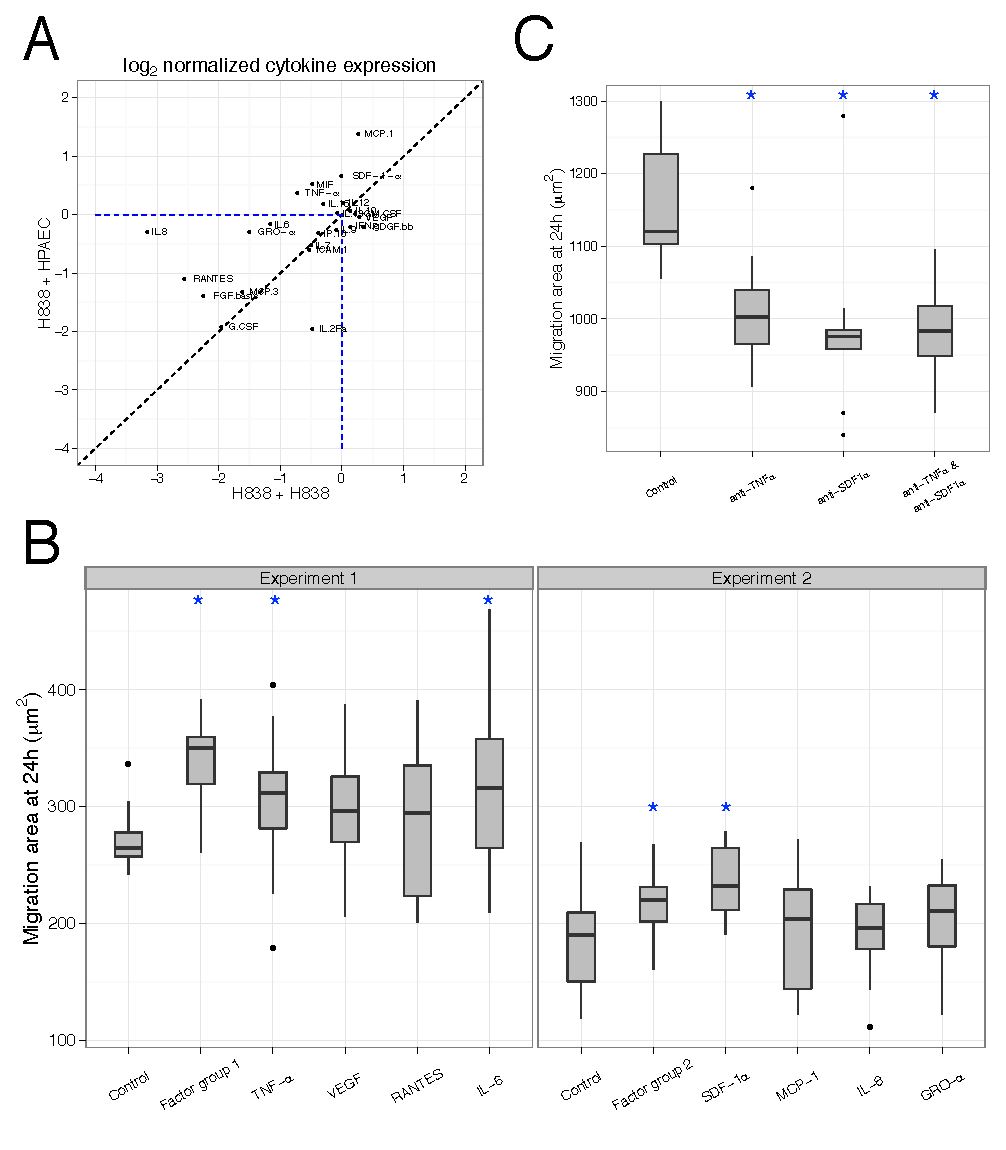
\includepdf[fitpaper=true]{fig/fig-cytokine.pdf}
%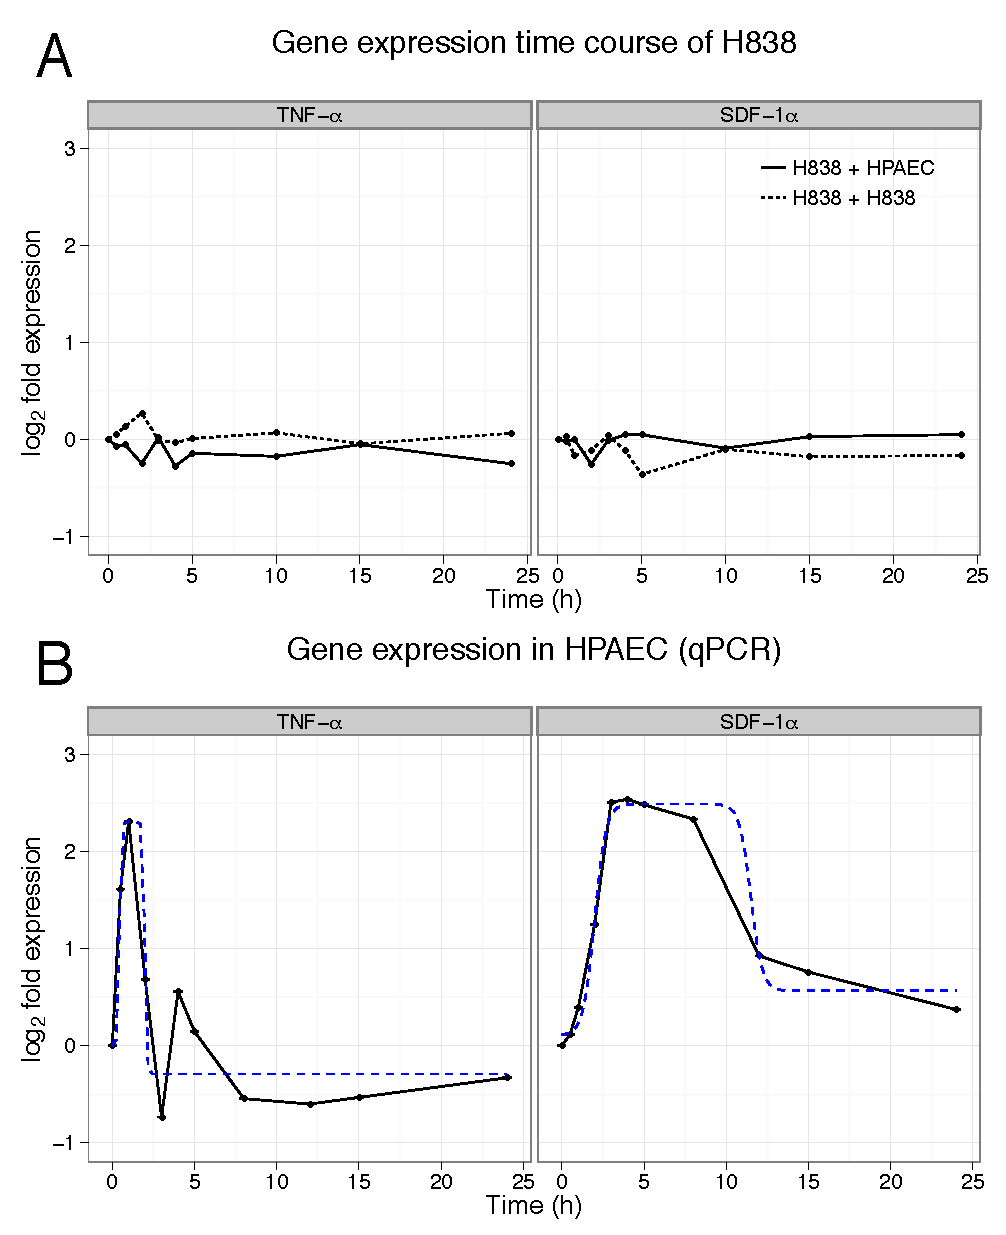
\includepdf[fitpaper=true]{fig/fig-cytokine_dynamic.pdf}
%\includepdf[fitpaper=true]{fig/fig-plot_tfbs_modified.pdf}
%\includepdf[fitpaper=true]{fig/fig-spl.pdf}
%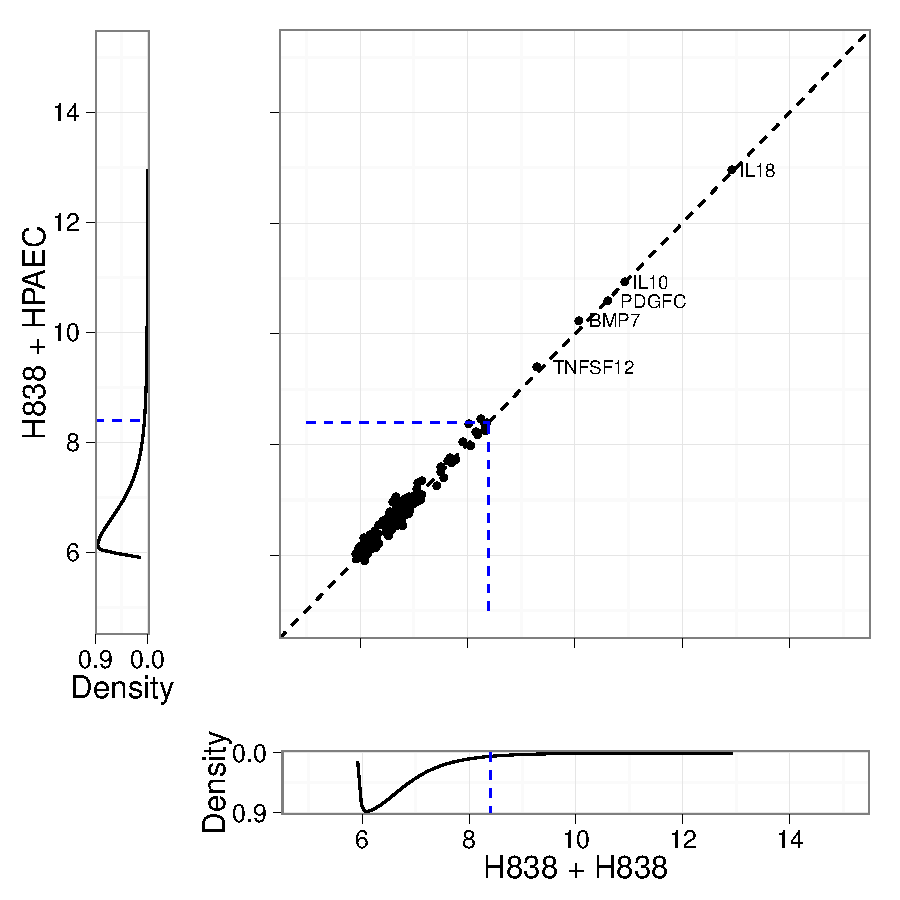
\includepdf[fitpaper=true]{fig/fig-basal_cytokine.pdf}

\section{Application in skin cell communication}




